%----------------------------------------------------------------------------------------
%   PACKAGES AND OTHER DOCUMENT CONFIGURATIONS
%----------------------------------------------------------------------------------------

\documentclass[12pt]{article}
\usepackage[english]{babel}
\usepackage[utf8x]{inputenc}
\usepackage{amsmath}
\usepackage{graphicx}
\usepackage{float}
\usepackage{mathtools}
\usepackage[colorinlistoftodos]{todonotes}

\begin{document}

\begin{titlepage}

\newcommand{\HRule}{\rule{\linewidth}{0.5mm}} % Defines a new command for the horizontal lines, change thickness here

\center % Center everything on the page
 
%----------------------------------------------------------------------------------------
%   HEADING SECTIONS
%----------------------------------------------------------------------------------------

%\textsc{\LARGE Uppsala University}\\[1.5cm] % Name of your university/college

\includegraphics[scale=.2]{images/fri_logo.png}\vspace{1.8cm}\\[1cm] % Include a department/university logo - this will require the graphicx package
\textsc{\Large Mathematical modeling}\\[0.5cm] % Major heading such as course name
\textsc{\large project assignment}\\[0.5cm] % Minor heading such as course title

%----------------------------------------------------------------------------------------
%   TITLE SECTION
%----------------------------------------------------------------------------------------

\HRule \\[0.4cm]
{ \huge  Hand-written numerals recognition}\\[0.4cm] % Title of your document
\HRule \\[1.5cm]
 
%----------------------------------------------------------------------------------------
%   AUTHOR SECTION
%----------------------------------------------------------------------------------------

\begin{minipage}{0.5\textwidth}
\begin{flushleft} \large
	\emph{Authors:}\\
	Andrej Hafner\\ % Your name
	Anže Mur\vspace{1 cm}\\ % Your name
\end{flushleft}

\begin{flushleft} \large
	\emph{Mentors:}\\
	as. dr. Damir Franetič\\ % Your name
	prof. dr. Nežka Mramor Kosta \vspace{0.7 cm}\\ % Your name
\end{flushleft}


\end{minipage}\\[2cm]

%----------------------------------------------------------------------------------------
%   DATE SECTION
%----------------------------------------------------------------------------------------

{\large \today}\\[2cm] % Date, change the \today to a set date if you want to be precise

\vfill % Fill the rest of the page with whitespace

\end{titlepage}

\tableofcontents
\newpage
\listoffigures
\newpage

\section{Problem introduction}
<<<<<<< HEAD
Handwritten numerals recognition  is the ability of a computer to receive and interpret handwritten input from sources such as paper documents, photographs and other medias. Early optical character recognition (OCR) may be traced to technologies involving telegraphy and creating reading devices for the blind and from that cause we received many good OCR methods. In past decade handwritten digit recognition (and other OCR methods) has become very important task in every day life. The reason for its increasing popularity is because of its enormous set of practical applications. Hand written digit recognition helps us to solve various complex problems and saves us a lot of time. We can see some of its everyday practical uses in automatic processing of bank checks, postal zip code recognition, signatures validation and many others.\\
=======
Handwritten numerals recognition  is the ability of a computer to receive and interpret handwritten input from sources such as paper documents, photographs and other media. Early optical character recognition (OCR) may be traced to technologies involving telegraphy and creating reading devices for the blind and from that cause we received many good OCR methods. In past decade handwritten digit recognition (and other OCR methods) has become very important task in every day life. The reason for its increasing popularity is because of its enormous set of practical applications. Hand written digit recognition helps us to solve various complex problems and saves us allot of time. We can see some of its everyday practical uses in automatic processing of bank checks, postal zip code recognition, signatures validation and many others.\\
>>>>>>> 65bca9402214a0165e6f0cf0287d0b77e5556f40
\newline
In our project assignment we had to tackle the problem with two different handwritten digit recognition methods- Least squares method and Singular-value decomposition (SVD) method.

\newpage
\section{Data collecting}
In order to use those two methods we had to collect some data. We needed a big enough data set so the recognition would work better and we would have enough testing samples.We created a template and pass it around to our acquaintances. The template format is very simple - we have ten squares and atop of every square there is a digit (from 0-9) a user should write to the center of the square.
%slika
\begin{figure}[h]
	\centering
	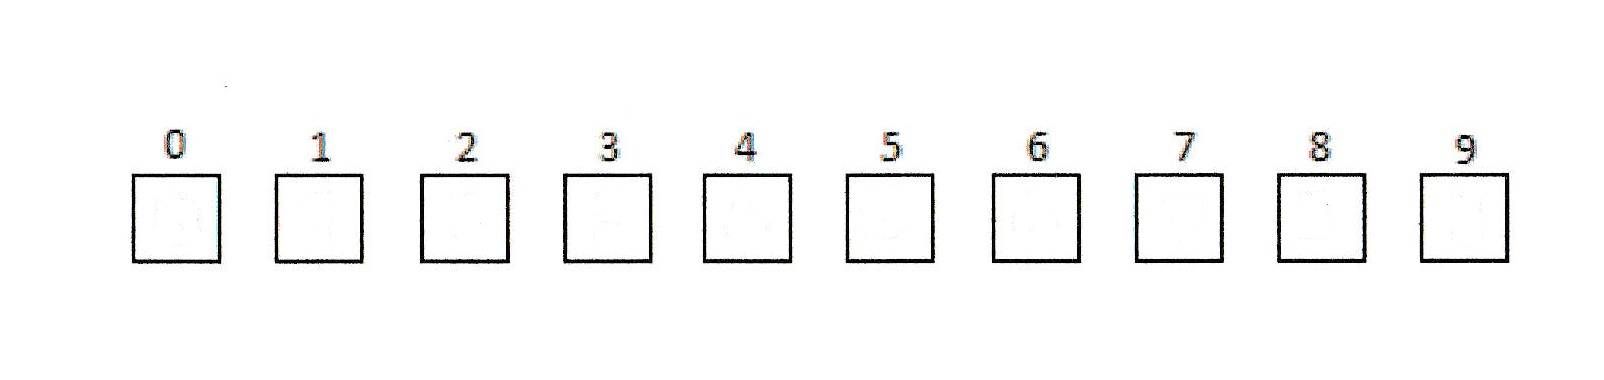
\includegraphics[clip,scale=0.62]{images/empty_temp.png}
	\caption[Data collection template]{Data collection template.}
	
\end{figure}
\newline
Our data collection was very successful and we gathered samples from 80 people (thats 800 handwritten digits). We soon realized that our data was not formated correctly. People have different style of writing so some of them didn't wrote the digits in the center of the square. That problem would significantly decrease the precision of the algorithms. Therefore we wrote a program in C++ using OpenCV libraries. It detects a square and cuts it out of an image and then computes the mass center of it. Then it creates a new square which is four times bigger than the original and pastes the the cut out square in the middle of the new square so that the mass center and the center of the big square are aligned. When the number is in place program computes the new angles of the square around the number and cuts it out of the big square. Now we have a perfectly aligned handwritten data piece.\\
\newline
We divided our data in two sets - training set and testing set. Most of the data (90\%) is in our training set and the rest (10\%) is in our testing set.\\

\newpage
%slika
\begin{figure}[h]
	\centering
	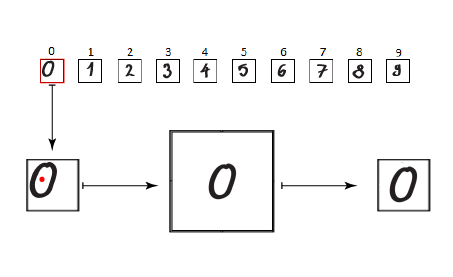
\includegraphics[clip,scale=0.9]{images/diagram.png}
	\caption[Process diagram of our C++ program]{Process diagram of our C++ program.}
	
\end{figure}



\newpage
\section{Used methods}
For our assignment we used two different methods for numeral handwritten recognition.
\subsection{Least squares method}
\textbf{About the method}\\
\newline
The method of least squares is a standard approach in regression analysis. We can approximate the solution of overdetermined systems that consists of sets of equations in which there are more equations than unknowns. Expression "least squares" means that the overall solution minimizes the sum of the squares and the errors made in the results of every single equation.\\
\newline
\textbf{Handwritten digit detection with least squares method:}



\begin{figure}[h]
	\centering
	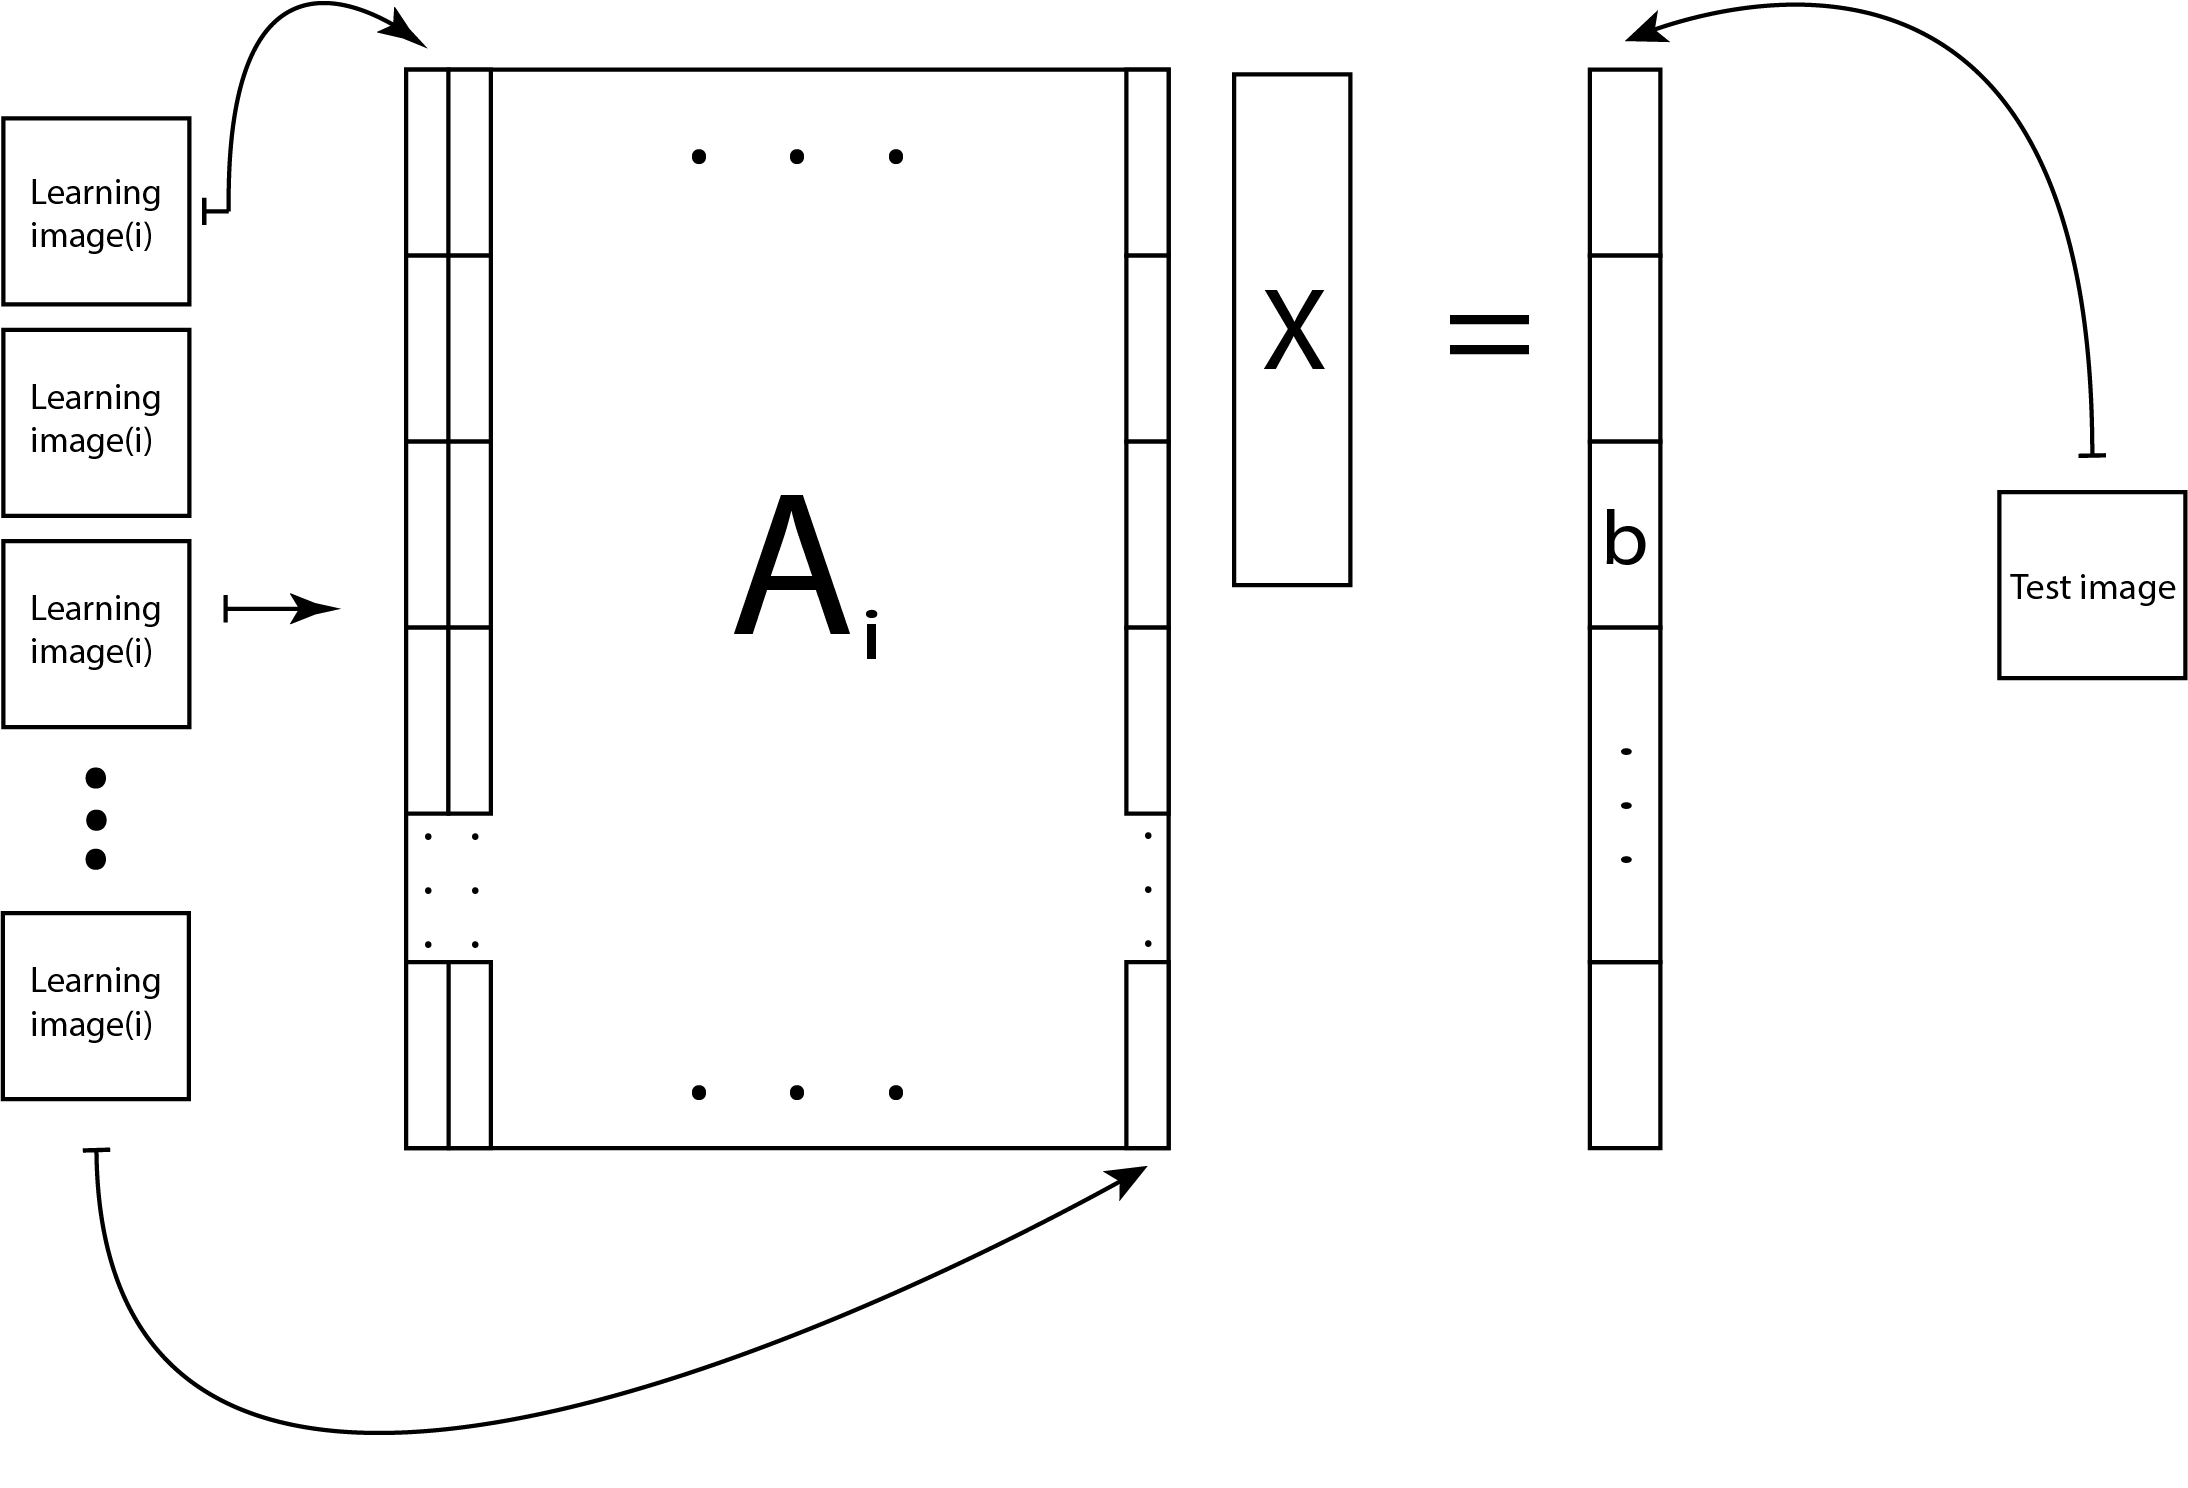
\includegraphics[clip,scale=0.68]{images/matrike.png}\underline{}
	\caption[Process diagram of least squares method matrix preparation]{Process diagram of least squares method matrix preparation.}
	
\end{figure}

\newpage
Let's say that we want know if one of our images from test set represents the digit $i$ (where $i = {0, 1, 2, 3, 4, 5, 6, 7, 8, 9}$ ).We take all of the images that represents digit $i$ from our learning set and we put them in a vector - we take every column from an image and we put them in the right order one under another. We do this for every image and we take those vectors and put them next to one another (as we can see on the diagram above) to construct a matrix \textbf{$A_{i}$}.\\
\newline
Now lets say that $b$ is a vector that represents our test image (we construct vector $b$ in the same way that we construct image vectors). Now we have a system $A_{i}x = b$. In general this system doesn't have a solution but we can solve it with the use of minimal norm - so we get the best approximation of the solution. We create the matrices $A_{i}$ for every digit from our learning set and we compute the solution of the system $x_{i} = A^{+}_{i}b$ for every $i$. Then we choose the $i$ for which the value of $|| b - A_{i}x_{i} ||$ is minimal. The $i$ that we get is the digit that we recognized.\\
\newline
You can see the implementation in file $digitRecognitionLeastSquares.m$.

\newpage
\subsection{Singular-value decomposition (SVD) method}
\textbf{About the method}\\
\newline
In linear algebra, the singular-value decomposition is a factorization of a real or complex matrix.
We define SVD of a matrix \textbf{A} as:\\
\[
A = U S V^{T}
\]
\newline
Where the matrices:
\begin{itemize}
	\item $U$: has columns that are the left singular vectors
	\item $S$: has singular values and is diagonal
	\item $V^{T}$: has rows that are the right singular vectors
\end{itemize}
The SVD represents the original data in a coordinate system where the covariance matrix is diagonal.\\
\newline
\textbf{Handwritten digit detection with SVD method:}\\
\newline
The least squares method is usually not really efficient and it takes allot of time to compute the answer. So it is better to use the SVD method. We prepare the data in the same way as before so that:
\begin{itemize}
	\item $A_{i}$ is our matrix built from learning images (for $i = 0, 1, 2, 3, 4, 5, 6, 7, 8, 9$),
	\item $b$ is our input/test image as a vector,
	\item and $x_{i}$ is solution we are looking for.
\end{itemize}
After we prepare our data we compute the singular value decomposition of the matrix $A_{i}$:\\
\[
A_{i} = U_{i} S_{i} V^{T}_{i}
\]
\newline
And then we search for solutions of the systems 
\[
U_{i} S_{i} y_{i} = b ;\quad \rlap{\text for every {$i$}}
\]
\newline
where:
\[
y_{i} = V^{T}_{i} x_{i}
\]\\
\newline
We get the solution in a similar way as before as we choose the $i$ for which the value of  \textbf{$|| U^{T}_{i} b - S_{i}y_{i} ||$}  is minimal.\\
\newline
You can see the implementation in file $digitRecognitionSvd.m$.

\newpage
\section{Theoretical basis}
We use the singular value decomposition to transform matrix $A_i$ into $U_iS_iV_i^{T}$. Digit recognition is the performed by solving finding solutions for systems of equations $U_iS_iy_i = b$, where $y_i = V^Tx_i$ and $b$ is the column vector of an image with the digit we are trying to recognize. The $U_i^{T}b - S_iy_i$ with the minimal norm is the solution and the digit recognized. \\
\newline
\textbf{Show that $||x_i|| = ||y_i||$} 
\newline
We use SVD on matrix $A$:

\[
A^{k \times p} = U^{k \times k}S^{k \times p}(V^T)^{p \times p}
\]
\newline
Where $p$ is the number of learning examples and $k$ equals $1024$ since our learning examples images were of size $32 \times 32$ and when we stack their columns one on top of another, we get a vector with dimension $1024 \times 1$. Then we stack these vectors next to eachother to create the matrix $A^{k \times p}$. \\
\newline
Because $y_i = V^Tx_i$ we get:
\newline
\[
 ||x_i^{p \times 1}|| = || (V^T)^{ p \times p} x_i^{p \times 1}||
\]
\newline
where $V^T$ (and also $U$) is a real unitary matrix, of which columns form a set of $orthonormal$ vectors. A set of vectors is orthonormal if they are $orthogonal$ to each other and are $unit$ vectors. An unit vector has a length of 1 and if you multiply a vector by an unit vector, it will only change it's direction, but not it's $norm$ (length). By the definition of a unitary matrix, the same is true for conjugate transposes of $V^T$ and $U$. This means that columns of $V$, $V^T$, $U$ and $U^T$ all form a set of orthonormal vectors. \\
\newline
We can conclude that multiplying $x_i$ by $V^T$ which results in $y_i$ will only change it's direction and not it's norm. Therefore it holds that $||x_i|| = ||y_i||$. \\
\newline
\textbf{Show that $||b - A_ix_i|| = ||U_i^{T}b - S_iy_i||$} \\
If we remove the norms from both sides of equation we get:\\

\[
b^{k \times 1} - A_i^{k \times p} x_i^{p \times 1} = (U_i^{T})^{k \times k}b^{k \times 1} - S_i^{k \times p}y_i^{p \times 1}
\]
\newline
where $k$ and $p$ have the same meaning as in the previous proof. Then we multiply the equation from the left side with $U_i^{k \times k}$ and use $y_i = V^Tx_i$. \\

\[
U_i^{k \times k}b^{k \times 1} - U_i^{k \times k}A_i^{k \times p} x_i^{p \times 1} = U_i^{k \times k}(U_i^{T})^{k \times k}b^{k \times 1} - U_i^{k \times k}S_i^{k \times p}(V_i^{T})^{p \times p}x_i^{p \times 1}
\]
\newline
Because $U$ is a unitary matrix, multiplying it by it's conjugate transpose yields an $identity$ matrix ($UU^T = I$). Multiplying a vector by an identity matrix will yield an identical vector. By removing the dimensions, using $A_i = U_iS_iV_i^{T}$ and the distributivity of matrix multiplication we can simplify the equation to: \\

\[
U_i(b - A_ix_i) = b - A_ix_i
\]
\newline
The matrix $U$ has columns that form a set of orthonormal vectors (further explanation in the previous proof). Multiplying a vector by $U$ will only change it's direction, but not the norm. This means that multiplying $b - A_ix_i$ by $U_i$ will not change it's norm. If we introduce back the norm on both sides we have shown that $||b - A_ix_i|| = ||U_i^{T}b - S_iy_i||$. \\
\[
||U_i(b - A_ix_i)|| = ||b - A_ix_i||
\]

\newpage
\section{Conclusion}

We used SVD to generate matrices $U$ $S$ and $V^T$. For recognition we can only store matrices $U$ and $S$. Because of the way that SVD works, the first $n$ singular values and left singular vectors hold most of the "patterns" or information needed for recognition. Because of this we can use only first $n$ singular values and left singular vectors for recognition, and still keep good accuracy at recognition. This means that we can only store those first $n$ values for each number. By doing this we reduce the size of the files (a file with U and V matrix for 80 learning examples can be as big as 10MB) and accelerate the calculation since there is less multiplication. We achieved best accuracy of 96\% when using 11 singular values. Using a lot of singular values can actually reduce the accuracy, since there is a lot of noise in the higher left singular vectors.



\end{document}